% TEX root = ../main.tex
\section{Implementación}
El montaje del sistema se realizó utilizando una placa de prototipos (protoboard) para facilitar la conexión de los componentes con la placa Arduino Uno, la cual actúa como unidad central de procesamiento.
El conexionado de los componentes, se realizó de la siguiente manera:

\begin{itemize}
    \item \textbf{Sensor DHT11}: La alimentación (VCC y GND) se conectó a los 5V y GND del Arduino. El pin de datos (DATA) se conectó al pin digital 9. 
    
    \item \textbf{Sensor GY-30 (BH1750FVI)}: Se conectó al bus I²C del Arduino. El pin VCC se conectó a 3.3V, GND a GND, el pin SCL (Serial Clock) al pin A5 y el pin SDA (Serial Data) al pin A4.
    
    \item \textbf{Pantalla Nextion}: Para asegurar un suministro de corriente estable, la alimentación de la pantalla se realizó de forma externa. La comunicación de datos se estableció conectando el pin RX de la pantalla al pin TX del Arduino (pin 1) y el pin TX de la pantalla al pin RX del Arduino (pin 0). Finalmente, se conectó el pin GND de la pantalla al GND del Arduino para establecer una referencia de tierra común.
\end{itemize}

\begin{figure}[H]
    \centering
    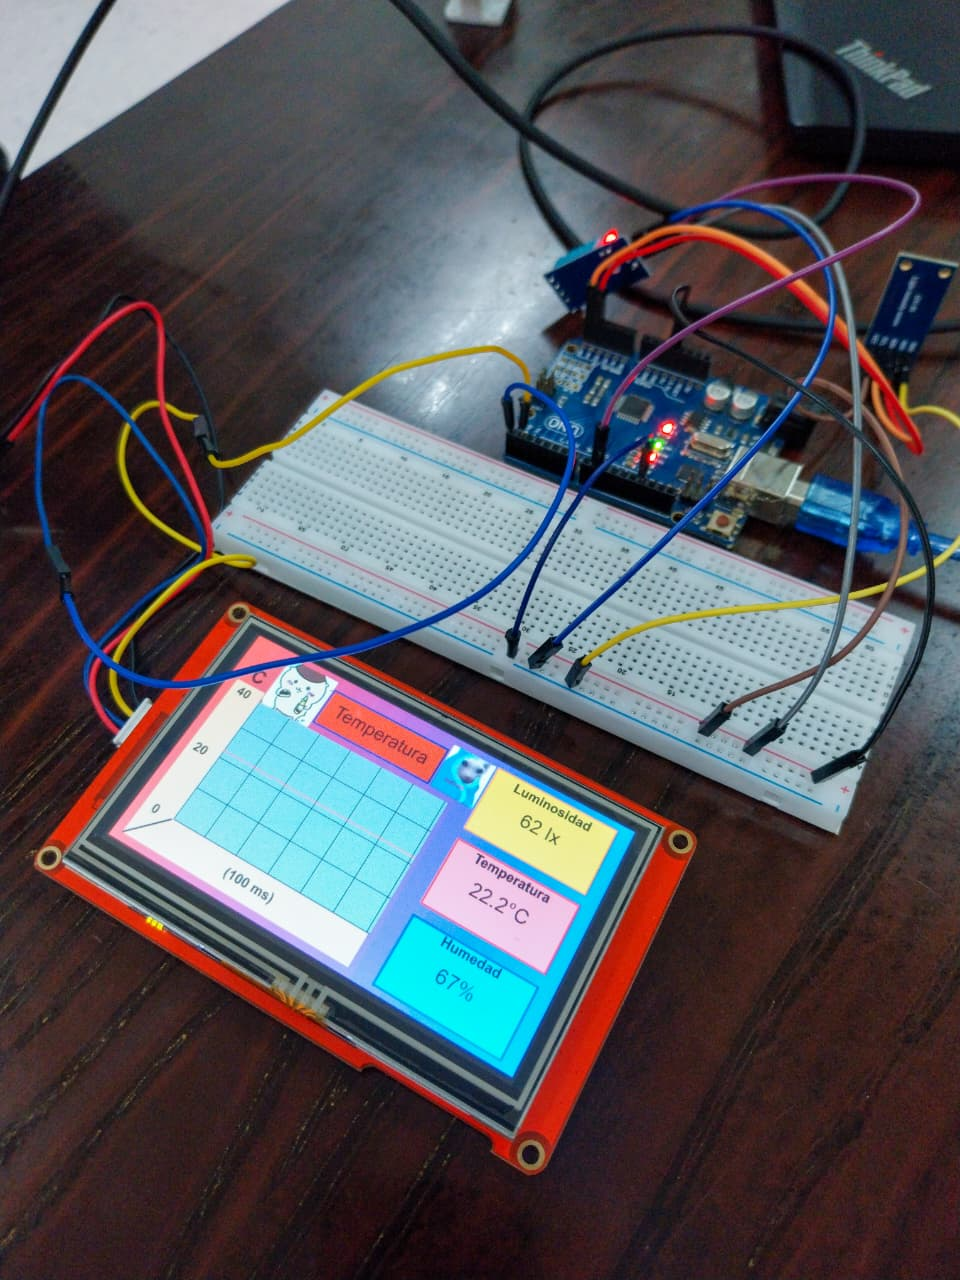
\includegraphics[width=0.6\textwidth]{Diagramas/impl.jpg} 
    \caption{Montaje físico del sistema de monitoreo ambiental.}
    \label{fig:montaje}
\end{figure}